\section{Epipolar geometry}

Epipolar geometry describes the relationship between two views of the same 3D scene. 
In the diagram below, the scene point, its projections, and the camera centers are coplanar, meaning the cameras' optical centers ($\mathbf{C}$ and $\mathbf{C}^\prime$), image points ($\mathbf{x}$ and $\mathbf{x}^\prime$), and the 3D scene point ($\mathbf{X}$) all lie on the same plane.
\begin{figure}[H]
    \centering
    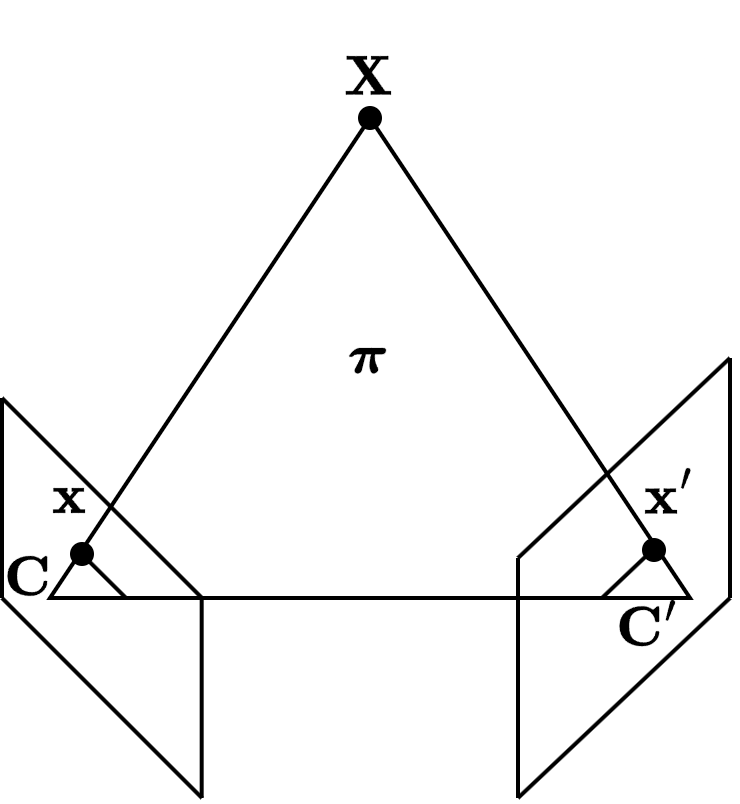
\includegraphics[width=0.5\linewidth]{images/epi.png}
    \caption{Epipolar geometry}
\end{figure}
The epipolar constraint states that the viewing rays corresponding to matching image points must intersect in 3D space. 
However, if only the camera centers and one image pointare known, the possible position of the 3D scene point lies somewhere along the viewing ray associated with the point. 

\paragraph*{Epipolar line}
The epipolar line is where the image of the 3D point varies along a line $\mathbf{l}^\prime$ in the second image.
Specifically, $\mathbf{l}^\prime$ is the image of the viewing ray, the line connecting the camera center to the 3D point.
The epipolar lines in both images correspond to each other and are related geometrically.
The viewing ray in the 3D space is a line through the first camera center. 
Therefore, its image in the second camera image plane, $\mathbf{l}^\prime$, always passes through the epipole $\mathbf{e}^\prime$, which is the projection of the first camera center in the second image.

\paragraph*{Epipolar constraint}
All points on the epipolar plane $\boldsymbol{\pi}$ project onto corresponding epipolar lines $\mathbf{l}$ and $\mathbf{l}^\prime$ in the two image planes.
The family of coaxial planes $\boldsymbol{\pi}$ where the baseline between the two cameras serves as the axis, intersects the image planes at the epipolar lines $\mathbf{l}$ and $\mathbf{l}^\prime$. 

The epipolar lines $\mathbf{l}$ and $\mathbf{l}^\prime$ converge at the epipoles $\mathbf{e}$ and $\mathbf{e}^\prime$, respectively.
These epipoles represent: 
\begin{itemize}
    \item The intersection of the baseline with the image plane.
    \item The projection of the camera centers in the other image.
    \item The vanishing point of the relative motion between the two cameras.
\end{itemize}

\begin{definition}[\textit{Epipolar plane}]
    A plane containing the baseline between the two cameras. 
    It defines a 1D family of planes that intersect the image planes in epipolar lines.
\end{definition}
\begin{definition}[\textit{Epipolar line}]
    The intersection of an epipolar plane with the image plane. 
    These lines come in corresponding pairs in each image and always pass through the epipoles.
\end{definition}
\begin{definition}[\textit{Epipolar points}]
    Points where the baseline intersects the image planes. 
    They are the projections of the camera centers in the opposite image and also serve as the vanishing points of the camera's relative motion direction.
\end{definition}

\subsection{Fundamental matrix}
The fundamental matrix provides an algebraic representation of the epipolar geometry between two views of a scene. 
It defines how points in one image correspond to lines in the other. This relationship can be described as follows:
\[\mathbf{x}\mapsto \mathbf{l}^\prime=\mathbf{Fx}\]
In this equation, $\mathbf{F}$ is the fundamental matrix, and it maps points from one image to corresponding epipolar lines in the other image.
This mapping is a form of correlation.

Mathematically, this is represented by the following expression:
\[\mathbf{F}=\begin{bmatrix}
    \mathbf{e}^\prime
\end{bmatrix}_{\times}\mathbf{M}^\prime\mathbf{M}^{-1}\mathbf{x}\]
Here, $\begin{bmatrix} \mathbf{e}^\prime \end{bmatrix}_{\times}$ is a skew-symmetric matrix used to compute the cross-product via matrix multiplication:
\[\begin{bmatrix} \mathbf{e}^\prime \end{bmatrix}_{\times}=\begin{bmatrix} 0 & -e^\prime_z & -e^\prime_y \\ e^\prime_z & 0 & -e^\prime_x \\ -e^\prime_y & e^\prime_x & 0 \end{bmatrix}\]
This matrix is singular, meaning it doesn't have an inverse.

The fundamental matrix satisfies a key condition: for any pair of corresponding points $(\mathbf{x},\mathbf{x}^\prime)$ in two images, the following equation holds:
\[\mathbf{x}^{\prime T}\mathbf{F}\mathbf{x}=\mathbf{0}\]
Here, $\mathbf{x}^\prime T\mathbf{l}^\prime=0$.
Even if the cameras are not calibrated and their projection matrices $\mathbf{P}$ and $\mathbf{P}^\prime$ are unknown, the fundamental matrix $\mathbf{F}$ can still be computed by using point correspondences between the two images.

\paragraph*{Properties}
The fundamental matrix has several important properties:
\begin{itemize}
    \item \textit{Uniqueness}: $\mathbf{F} = \begin{bmatrix} \mathbf{e}^\prime \end{bmatrix}_{\times} \mathbf{M}^\prime \mathbf{M}^{-1}$ is the only $3\times 3$ matrix with rank two that satisfies $\mathbf{x}^{\prime T} \mathbf{F} \mathbf{x} = 0$ for all corresponding points $\mathbf{x} \leftrightarrow \mathbf{x}^\prime$.
    \item \textit{Transpose property}: if $\mathbf{F}$ is the fundamental matrix for the camera pair $(\mathbf{P}, \mathbf{P}^\prime)$, then $\mathbf{F}^T$ is the fundamental matrix for the reversed camera pair $(\mathbf{P}^\prime, \mathbf{P})$.
    \item \textit{Epipolar lines}: the epipolar line corresponding to a point $\mathbf{x}$ in the first image is given by $\mathbf{l} = \mathbf{F} \mathbf{x}$, and the epipolar line corresponding to a point $\mathbf{x}^\prime$ in the second image is $\mathbf{l}^\prime = \mathbf{F}^T \mathbf{x}^\prime$.
    \item \textit{Epipoles}: the epipoles are the points where all the epipolar lines converge. 
        They lie on the null space of $\mathbf{F}$. 
        Thus, $\mathbf{e}^{\prime T} \mathbf{F} = 0$ and $\mathbf{F} \mathbf{e} = 0$, where $\mathbf{e}$ and $\mathbf{e}^\prime$ are the epipoles in the first and second image, respectively.
    \item \textit{Degrees of freedom}: the fundamental matrix has 7 degrees of freedom, as it is a $3\times 3$ matrix with $9$ elements, but constrained by the rank-2 condition and the homogeneous coordinate system (removing 2 degrees of freedom).
    \item \textit{Projective mapping}: the fundamental matrix represents a projective mapping from a point in one image to a line in the other image. 
        This is not a proper correlation because the mapping is not invertible.
\end{itemize}

\paragraph*{Computation}
To compute the fundamental matrix $\mathbf{F}$ from a set of corresponding image points, we solve the following system of equations:
\[\mathbf{F}\mathbf{x}_i=0\]
These equations are linear in the elements of $\mathbf{F}$, and the matrix can be computed using various methods. 
The most common approaches are:
\begin{itemize}
    \item Using 8 point pairs, which provides a linear system of equations.
    \item Using 7 point pairs, which gives a non-linear system.
    \item Using 8 or more point pairs and solving the system using least squares optimization.
\end{itemize}